\chapter{Results and Discussion}
\label{ch:results}

\section{Experimental Setup}

Every result in this chapter was produced on the testbed described in
Chapter~\ref{ch:methodology}: a single-node Minikube cluster (2 vCPU,
3\,GB RAM) on a MacBook Air M1 with 8\,GB RAM, running the benchmark
service of Section~\ref{sec:mdp} behind the deterministic traffic
generator of Section~\ref{sec:mdp}. We report V1's results first, then the
V2 training campaign, then the V2 pre-registered evaluation, then the
exploratory stress test, and close with a comparative analysis against the
related work of Chapter~\ref{ch:introduction} and a plain statement of
this project's limitations.

\section{V1 Results}

\subsection{V1 Evaluation}

V1's held-out evaluation ran three PPO episodes alternated with three HPA
episodes (order PPO1, HPA1, PPO2, HPA2, PPO3, HPA3) against a single
held-out traffic profile (seed 777, 1,500 seconds, 50 decision steps,
peaking at 65 requests per second). Table~\ref{tab:v1-eval-results}
reproduces the per-run results from the project's own V1 evaluation
ledger and analysis (\texttt{results/\allowbreak \allowbreak evaluation/\allowbreak \allowbreak }).

\begin{table}[H]
\centering
\caption{V1 held-out evaluation: per-run results. PPO1 and PPO2 ended in a safety termination (\texttt{consecutive\_\allowbreak invalid\_\allowbreak steps\_\allowbreak limit\_\allowbreak reached}) before completing all 50 decisions; PPO3 was the only PPO run to complete the full episode.}
\label{tab:v1-eval-results}
\small
\resizebox{\linewidth}{!}{%
\begin{tabular}{lrrrrr}
\toprule
Run & Steps completed & SLA-viol.\ rate (300\,ms) & Mean p95 (ms) & Mean replicas & Scaling actions \\
\midrule
PPO1 (terminated) & 23/50 & 0.83 & 1925 & 0.75 & 0 \\
HPA1 & 50/50 & 0.72 & 1592 & 5.06 & 10 \\
PPO2 (terminated) & 20/50 & 0.70 & 2024 & 0.67 & 0 \\
HPA2 & 50/50 & 0.54 & 987 & 5.35 & 14 \\
PPO3 (valid) & 50/50 & 0.92 & 2298 & 1.20 & 3 \\
HPA3 & 50/50 & 0.52 & 689 & 5.29 & 15 \\
\bottomrule
\end{tabular}%
}
\end{table}

No run of either controller produced any 5xx errors. PPO's one valid
repeat (PPO3) used far fewer replicas on average than any HPA run (1.20
versus 5.06-5.35), which is the behaviour V1's unconditional resource cost
(Equation~\ref{eq:v1-reward}) was designed to encourage, but its latency
and SLA-violation rate were clearly worse than every HPA run: mean p95
latency of 2,298\,ms against an HPA range of 689-1,592\,ms, and an
SLA-violation rate of 0.92 against an HPA range of 0.52-0.72. Because the
pre-registered rule for this evaluation required three valid repeats per
controller and PPO produced only one, no winner could be declared between
PPO and HPA under V1 -- the evaluation correctly refused to produce a
verdict from two-thirds-missing data, rather than reporting PPO3's single
result as if it represented the policy's typical behaviour.

\begin{sloppypar}
\textit{V1-era figures.} The V1 figures referenced by this project's own
figure index predate the V2 figure-generation pipeline and are not stored
under \texttt{docs/\allowbreak \allowbreak archive/\allowbreak \allowbreak figures\_\allowbreak v1/\allowbreak \allowbreak }, which exists in the repository
but is empty. The actual V1 evaluation figures were located instead under
\texttt{results/\allowbreak \allowbreak figures/\allowbreak \allowbreak } (added in the project's first commit, before any
V2 work existed): \texttt{final\_\allowbreak mean\_\allowbreak p95\_\allowbreak latency.png},
\texttt{final\_\allowbreak mean\_\allowbreak replicas.png}, \texttt{final\_\allowbreak sla\_\allowbreak violation\_\allowbreak rate.png},
\texttt{final\_\allowbreak action\_\allowbreak churn.png}, \texttt{final\_\allowbreak reaction\_\allowbreak time.png},
\texttt{final\_\allowbreak resource\_\allowbreak proxy.png}, \texttt{evaluation\_\allowbreak outcomes.png},
\texttt{p95\_\allowbreak latency\_\allowbreak over\_\allowbreak time\_\allowbreak full\_\allowbreak runs.png}, and
\texttt{replicas\_\allowbreak over\_\allowbreak time\_\allowbreak full\_\allowbreak runs.png}. Figure~\ref{fig:v1-replicas}
and Figure~\ref{fig:v1-p95} reproduce the two time-series figures from this
set.
\end{sloppypar}

\begin{figure}[htbp]
\centering
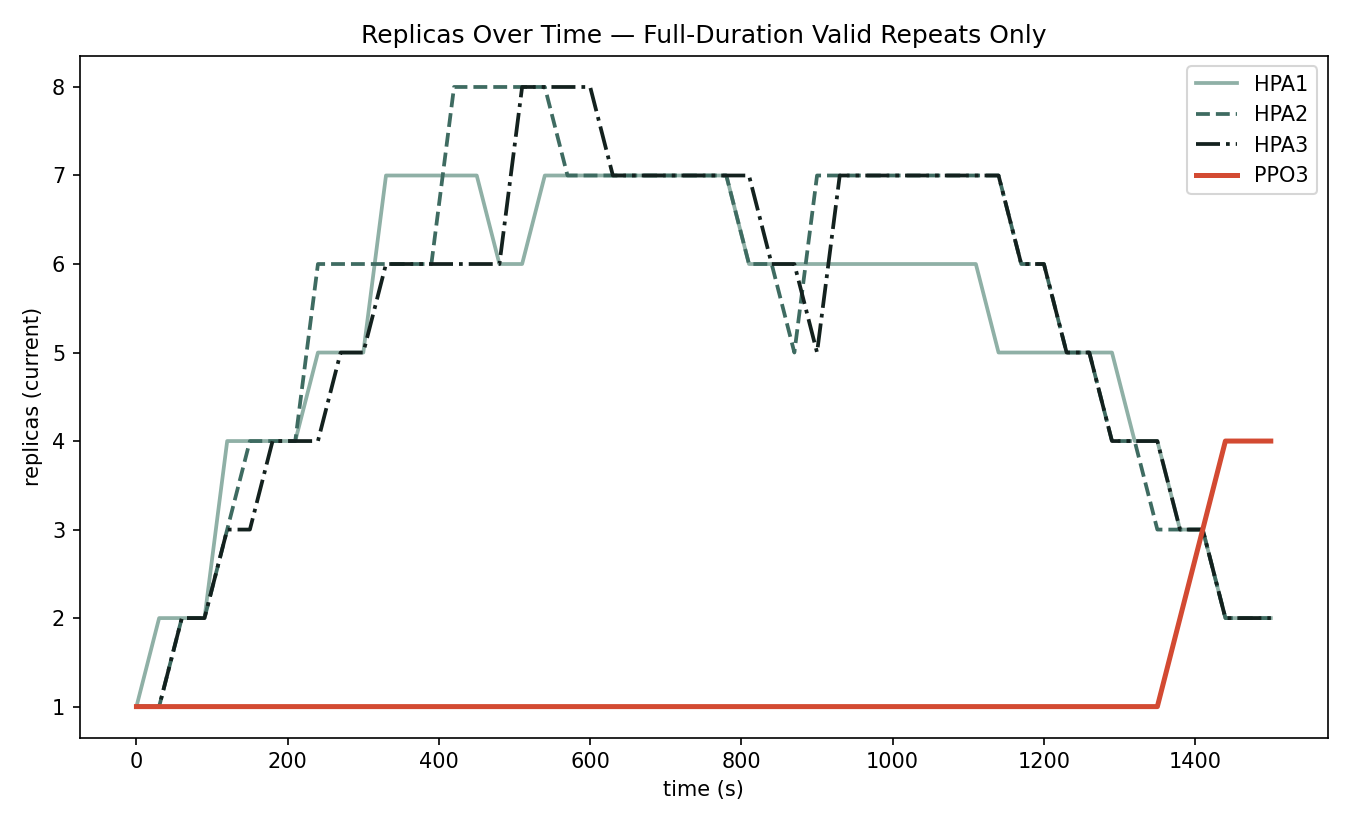
\includegraphics[width=0.42\textwidth]{../../results/figures/replicas_over_time_full_runs.png}
\caption{V1: replica count over time across the three full (non-terminated) runs of the held-out evaluation episode. Source: \texttt{results/\allowbreak \allowbreak figures/\allowbreak \allowbreak replicas\_\allowbreak over\_\allowbreak time\_\allowbreak full\_\allowbreak runs.png}.}
\label{fig:v1-replicas}
\end{figure}

\begin{figure}[htbp]
\centering
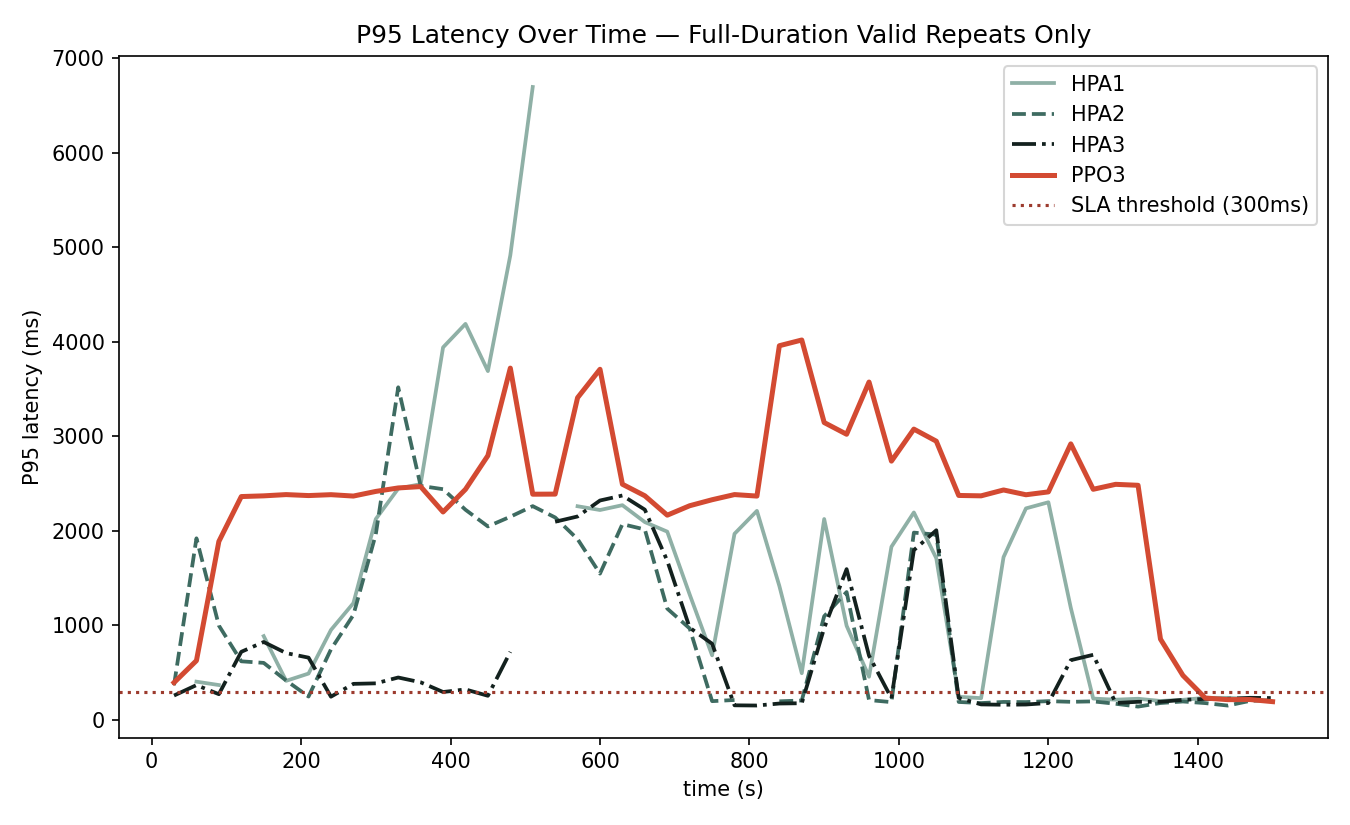
\includegraphics[width=0.42\textwidth]{../../results/figures/p95_latency_over_time_full_runs.png}
\caption{V1: p95 latency over time across the three full (non-terminated) runs of the held-out evaluation episode. Source: \texttt{results/\allowbreak \allowbreak figures/\allowbreak \allowbreak p95\_\allowbreak latency\_\allowbreak over\_\allowbreak time\_\allowbreak full\_\allowbreak runs.png}.}
\label{fig:v1-p95}
\end{figure}

\subsection{V1 Failure Analysis}
\label{sec:v1-failure}

Two of PPO's three evaluation runs (PPO1, PPO2) ended in a safety
termination triggered by \texttt{consecutive\_\allowbreak invalid\_\allowbreak steps\_\allowbreak limit\_\allowbreak reached}
roughly 10-11.5 minutes into their respective episodes, well after real
traffic had already been flowing continuously -- ruling out a one-off
cold-start telemetry gap as the explanation. We identified two design
decisions, both in V1 and both corrected in V2, that together explain this
pattern. First, V1's resource term in Equation~\ref{eq:v1-reward},
$-(n_t-1)/7$, charges a cost for every replica above one on every single
step, regardless of whether those replicas are doing anything useful; this
creates a persistent incentive to stay at the smallest possible replica
count even when load genuinely calls for more capacity. Second, V1's
replica floor of one meant that, once the policy had been driven toward a
single replica, that one pod's own saturation or a transient restart could
take the Deployment's entire ready-replica count to zero with no structural
redundancy to fall back on -- and a sustained loss of ready replicas is
exactly the condition that feeds \texttt{consecutive\_\allowbreak invalid\_\allowbreak steps}
toward its termination limit, since no telemetry can be attributed to a
pod that does not exist. A separate, SB3-default artefact compounds this:
deterministic inference's arg-max tie-break resolves an uncertain policy
toward the lowest action index, which in our action encoding is
\textsc{scale\_down\_one} -- so an uncertain V1 policy was silently biased
toward removing capacity even when it was not confidently the best choice,
never because removing capacity was actually assessed as correct. These
three findings -- an unconditional resource cost, a replica floor with no
redundancy, and a tie-break rule that silently favours scaling down -- are
precisely the three design points changed first in the V2 redesign of
Section~\ref{sec:v1-to-v2}.

\section{V2 Training Campaign}

\subsection{Learning Curves}

Figure~\ref{fig:training-reward} through Figure~\ref{fig:training-action-mix}
show the V2 training campaign's learning indicators across all 48 analyzed
sessions (12,288 cumulative timesteps). Dashed vertical markers in each
figure indicate sessions 4 and 38, the two sessions that failed and were
retried (Section~\ref{sec:zero-ready-stops}).

\begin{figure}[htbp]
\centering
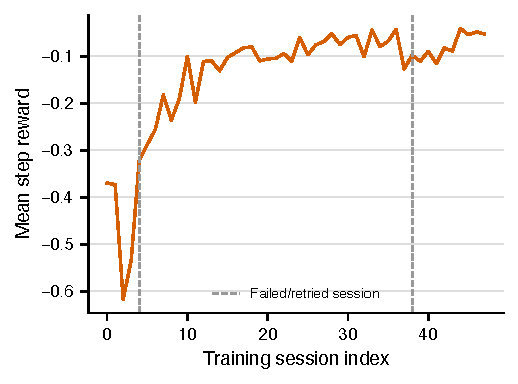
\includegraphics[width=0.42\textwidth]{../figures/training_mean_step_reward.pdf}
\caption{Mean per-step reward per training session, 48 sessions; dashed lines mark sessions 4 and 38 (failed, retried).}
\label{fig:training-reward}
\end{figure}

\begin{figure}[htbp]
\centering
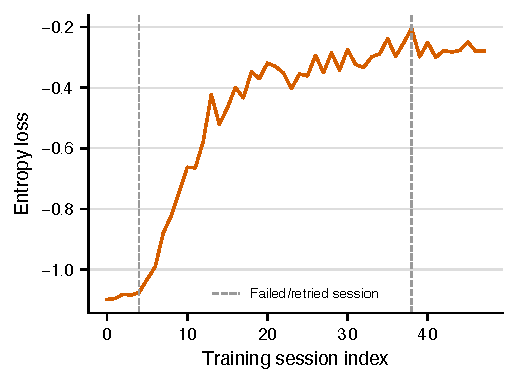
\includegraphics[width=0.42\textwidth]{../figures/training_entropy.pdf}
\caption{Policy entropy loss per training session, 48 sessions; dashed lines mark sessions 4 and 38.}
\label{fig:training-entropy}
\end{figure}

\begin{figure}[htbp]
\centering
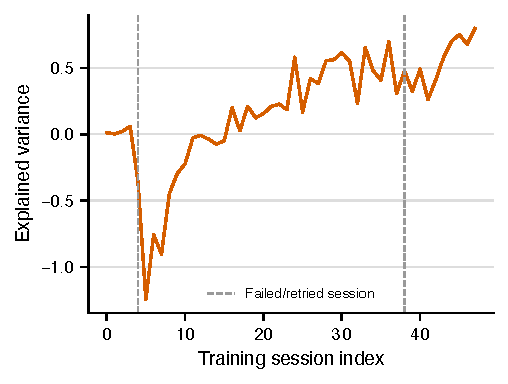
\includegraphics[width=0.42\textwidth]{../figures/training_explained_variance.pdf}
\caption{Explained variance of the value function per training session, 48 sessions; dashed lines mark sessions 4 and 38.}
\label{fig:training-ev}
\end{figure}

\begin{figure}[htbp]
\centering
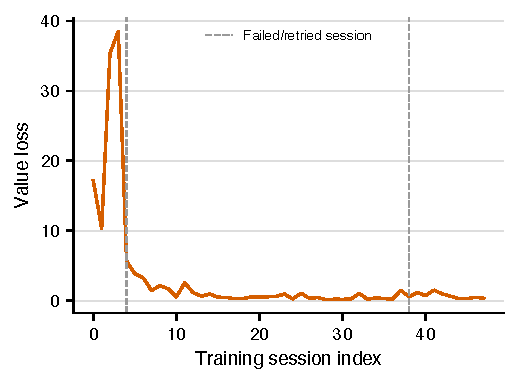
\includegraphics[width=0.42\textwidth]{../figures/training_value_loss.pdf}
\caption{Value loss per training session, 48 sessions; dashed lines mark sessions 4 and 38.}
\label{fig:training-vloss}
\end{figure}

\begin{figure}[htbp]
\centering
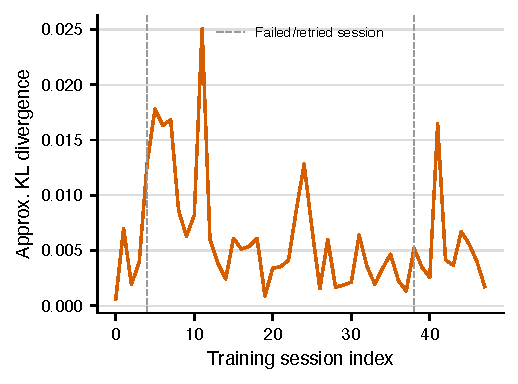
\includegraphics[width=0.42\textwidth]{../figures/training_approx_kl.pdf}
\caption{Approximate KL divergence per PPO update, 48 sessions; dashed lines mark sessions 4 and 38.}
\label{fig:training-kl}
\end{figure}

\begin{figure}[htbp]
\centering
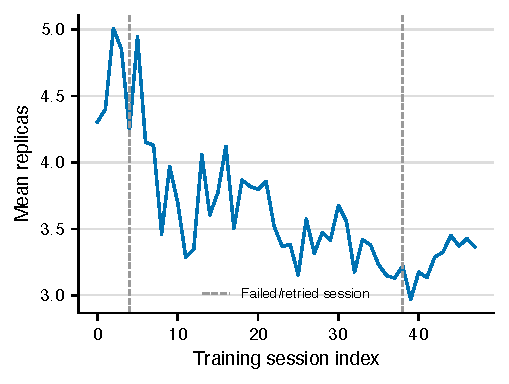
\includegraphics[width=0.42\textwidth]{../figures/training_mean_replicas.pdf}
\caption{Mean replica count per training session, 48 sessions; dashed lines mark sessions 4 and 38.}
\label{fig:training-replicas}
\end{figure}

\begin{figure}[htbp]
\centering
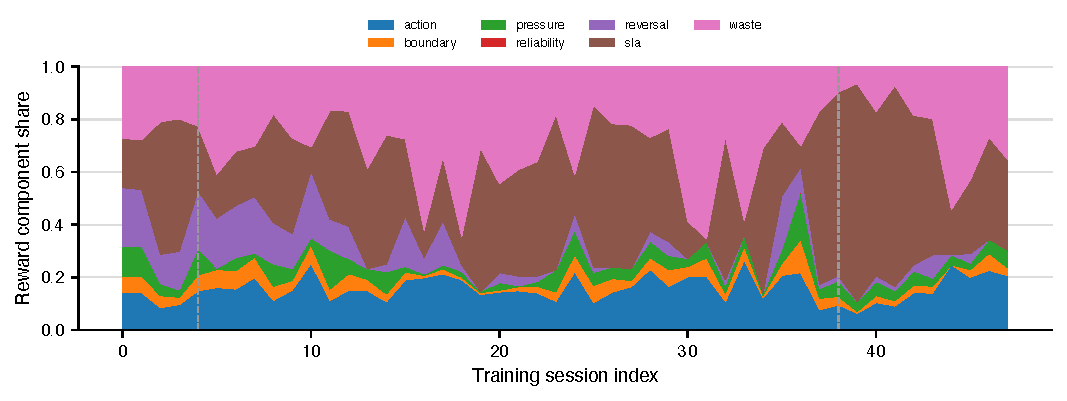
\includegraphics[width=0.42\textwidth]{../figures/training_reward_components.pdf}
\caption{Relative share of each reward component (by absolute mean value) per training session, 48 sessions; dashed lines mark sessions 4 and 38.}
\label{fig:training-components}
\end{figure}

\begin{figure}[htbp]
\centering
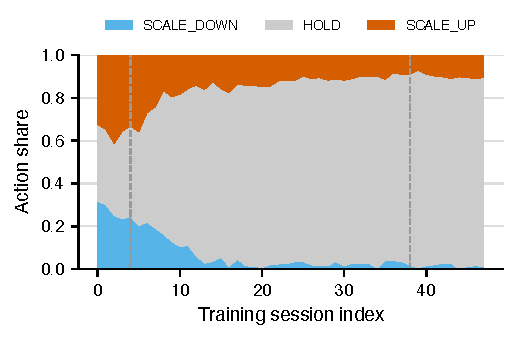
\includegraphics[width=0.42\textwidth]{../figures/training_action_mix.pdf}
\caption{Fraction of SCALE\_DOWN/HOLD/SCALE\_UP actions per training session, 48 sessions; dashed lines mark sessions 4 and 38.}
\label{fig:training-action-mix}
\end{figure}

Table~\ref{tab:training-summary} summarizes the key endpoints: entropy
loss, which measures how random the policy's action distribution is, falls
from $-1.0984$ at the first analyzed session to $-0.2792$ at the last,
consistent with the policy becoming progressively less random (more
confident in its choices) over the campaign. Explained variance of the
value function -- the fraction of the variance in observed returns that
the value function's predictions account for, with 1.0 meaning perfect
prediction and 0 meaning no better than predicting the mean -- rises from
0.0125 at the very first PPO update to a mean of 0.703 over the final five
updates (sessions 43-47), peaking at 0.799, computed directly from
\texttt{persistent-data/\allowbreak \allowbreak rl\_\allowbreak training\_\allowbreak v2/\allowbreak \allowbreak final\_\allowbreak min2/\allowbreak \allowbreak ppo\_\allowbreak update\_\allowbreak metrics.jsonl}.
This rise is not perfectly monotonic: the same underlying data shows a
minimum explained variance of $-1.2461$ at some point after the first
update (Table~\ref{tab:training-summary}), meaning the value function's
predictions were, briefly, worse than simply predicting the mean return --
consistent with PPO's on-policy updates occasionally destabilizing the
value function's fit before it recovers, which is a known and generally
tolerated property of on-policy actor-critic training rather than a sign
that training failed.

\begin{table}[H]
\centering
\caption{V2 training summary: key endpoints across 48 analyzed sessions.}
\label{tab:training-summary}
\begin{tabular}{ll}
\hline
field & value \\
\hline
n\_sessions\_analyzed & 48 \\
first\_session\_entropy\_loss & -1.0984 \\
last\_session\_entropy\_loss & -0.2792 \\
min\_entropy\_loss & -1.0984 \\
max\_entropy\_loss & -0.2048 \\
first\_session\_explained\_variance & 0.0125 \\
last\_session\_explained\_variance & 0.7993 \\
min\_explained\_variance & -1.2461 \\
max\_explained\_variance & 0.7993 \\
n\_failed\_retried\_attempts & 2 \\
failed\_attempt\_session\_indices & 4, 38 \\
\hline
\end{tabular}

\end{table}

\subsection{Training Progression}

Reading the same underlying curves as a progression rather than only as
endpoints: mean step reward improves steadily across the campaign, the
HOLD action's share of all decisions rises as the policy learns to avoid
unnecessary scaling churn, and mean replica count drifts downward from an
early-campaign level toward the lower half of the 2-8 replica range,
consistent with the policy learning that most of the training traffic
profiles do not need many replicas to keep latency and error rate healthy.
This progression is visible directly in
Figures~\ref{fig:training-reward}-\ref{fig:training-action-mix} and is the
basis for the discussion of what the policy had and had not converged to
by session 47 in Section~\ref{sec:discussion}.

\subsection{The Two Zero-Ready-Pod Stops}
\label{sec:zero-ready-stops}

Two of the campaign's 48 planned sessions failed on their first physical
attempt and had to be resumed from the previous checkpoint: session 4 and
session 38. Both failures share the identical recorded reason,
\texttt{zero\_\allowbreak ready\_\allowbreak replicas}, read directly from each session's own
\texttt{SESSION\_\allowbreak FAILED.json}: session 4 failed after completing 126 of
its planned 256 steps, and session 38 after completing 163 of 256. In both
cases, every ready replica of the Deployment dropped to zero during the
session -- the same structural failure mode diagnosed for V1 in
Section~\ref{sec:v1-failure}, except that by this point in the V2 campaign
the replica floor had already been raised to 2 (CORR-55), so this is not a
recurrence of the single-replica vulnerability itself; it reflects that a
floor of 2 reduces, but does not eliminate, the chance that correlated pod
unhealthiness (for example, both replicas restarting close together under
load) can still, on rare occasions, take ready-replica count to zero. Both
sessions were resumed from their last good checkpoint using the
session/checkpoint/resume design of Chapter~\ref{ch:methodology}, each
completing successfully as session \texttt{\_\allowbreak \_\allowbreak attempt2}, which is why the
campaign's 48 analyzed sessions are complete, successful retries and not a
silently dropped or averaged-over set of failures; both are marked
explicitly with dashed lines in every learning-curve figure in this
section.

A closely related event, worth reporting plainly rather than omitting, is
documented in the project's own Phase 5E report: partway through an
unrelated, offline user-interface development task, a routine, read-only
process check found that the live training campaign's process (PID 26490)
had disappeared. Reading the campaign's own metadata file showed the
campaign had stopped itself at session 4 on the \texttt{zero\_\allowbreak ready\_\allowbreak replicas}
condition described above, with sessions 0-3 already safely checkpointed;
no command from that phase, or any other phase, had touched the cluster,
the lock file, or the training process at any point, and the project's own
established discipline was followed: no restart or retry was attempted
until the stoppage had been reviewed. \textbf{[CHECK]}: our search of this
project's documentation did not turn up a separately confirmed incident in
which the V2 training process itself was killed by an external signal
(as distinct from the self-terminating \texttt{zero\_\allowbreak ready\_\allowbreak replicas}
stops at sessions 4 and 38 described above); if such an externally-killed
re-run occurred, we were not able to locate its record in the materials
available to us and flag this explicitly rather than asserting a cause we
could not verify.

\section{Pre-Registered Evaluation}

\subsection{Overview}

The pre-registered \texttt{eval\_\allowbreak final} campaign (CORR-60) ran all 27
planned attempts (3 profiles $\times$ 3 arms $\times$ 3 repeats) to a
VALID outcome. No run ended in a safety termination; no pod restarted
during any of the 27 runs (\texttt{pod\_\allowbreak restarts\_\allowbreak total == 0} throughout).
Four attempts failed on their first try due to a leftover HPA object from
the previous arm's run blocking controller acquisition (CORR-63, CORR-64)
and were retried once each under the tooling-failure rule of
Section~\ref{sec:eval-protocol}, with zero effect on the measured result
once retried; this is reported here rather than silently absorbed into the
27 VALID figures, consistent with this project's discipline of preserving
every attempt's evidence, successful or not.

\subsection{Primary Metrics}

Table~\ref{tab:eval-primary} reports the primary metrics, mean $\pm$
standard deviation over the three repeats of each (profile, arm) cell.

\begin{table}[H]
\centering
\caption{\texttt{eval\_\allowbreak final} primary metrics: SLA-violation rate at the 1000\,ms target and replica-minutes, mean $\pm$ sd over 3 repeats.}
\label{tab:eval-primary}
\small
\resizebox{\linewidth}{!}{\begin{tabular}{lllll}
\hline
profile & arm & n\_repeats & sla\_violation\_rate\_1000ms & replica\_minutes \\
\hline
CPU step & HPA CPU+Memory (resource baseline) & 3 & 0.0000 +/- 0.0000 & 60.5000 +/- 0.8660 \\
CPU step & HPA CPU-only (CPU baseline) & 3 & 0.0000 +/- 0.0000 & 59.3333 +/- 0.2887 \\
CPU step & PPO (multi-metric, 11 signals) & 3 & 0.0083 +/- 0.0144 & 72.6667 +/- 0.2887 \\
memory ramp & HPA CPU+Memory (resource baseline) & 3 & 0.0000 +/- 0.0000 & 75.1667 +/- 1.6073 \\
memory ramp & HPA CPU-only (CPU baseline) & 3 & 0.0000 +/- 0.0000 & 40.0000 +/- 0.0000 \\
memory ramp & PPO (multi-metric, 11 signals) & 3 & 0.0000 +/- 0.0000 & 56.1667 +/- 0.2887 \\
mixed bursts & HPA CPU+Memory (resource baseline) & 3 & 0.0000 +/- 0.0000 & 74.6667 +/- 5.1316 \\
mixed bursts & HPA CPU-only (CPU baseline) & 3 & 0.0000 +/- 0.0000 & 40.0000 +/- 0.0000 \\
mixed bursts & PPO (multi-metric, 11 signals) & 3 & 0.0000 +/- 0.0000 & 58.3333 +/- 2.3094 \\
\hline
\end{tabular}
}
\end{table}

Under our pre-registered decision rule (Table~\ref{tab:decision-rule}: an
arm is "better" on a metric for a profile only if it wins in all three of
three repeats), the SLA-violation rate at the 1000\,ms target does not
produce a decidable winner for any arm pair on any profile -- every arm
sits at or extremely close to its floor of 0.0 on every profile, with the
one exception of PPO on \texttt{eval\_\allowbreak cpu\_\allowbreak step} (mean 0.0083, i.e.\ a
single decision out of 360 total PPO decisions breached the SLA across the
whole campaign), which is itself too close to zero, and too inconsistent
across repeats ($\pm 0.0144$), to support a "better" claim either way.
Replica-minutes (our cost proxy) does discriminate, but not in favour of a
single arm: the HPA CPU-only (CPU baseline) arm is cheapest on
\texttt{eval\_\allowbreak memory\_\allowbreak ramp} (40.0 versus PPO's 56.17 and the HPA
CPU+Memory arm's 75.17) and on \texttt{eval\_\allowbreak mixed\_\allowbreak burst} (40.0 versus
58.33 and 74.67), and effectively ties with HPA CPU+Memory on
\texttt{eval\_\allowbreak cpu\_\allowbreak step} (59.33 versus 60.5, both cheaper than PPO's
72.67). PPO is therefore the most expensive arm on \texttt{eval\_\allowbreak cpu\_\allowbreak step}
but the cheapest of the three arms on the other two profiles besides the
CPU-only baseline -- a profile-dependent cost ranking, not a uniform one,
exactly the kind of outcome our decision rule is built to report as a
trade-off rather than resolve into a single ranking.

\subsection{Secondary Metrics}

Table~\ref{tab:eval-secondary-main} reports mean p95 latency and maximum
per-pod memory for each cell; the full secondary-metrics table, including
error rate, scaling-action and reversal counts, and the 300\,ms reference
SLA rate, is given in Appendix~\ref{ch:appendix},
Table~\ref{tab:eval-secondary-appendix}.

\begin{table}[H]
\centering
\caption{\texttt{eval\_\allowbreak final} secondary metrics (selected columns): mean p95 latency and maximum per-pod memory, mean $\pm$ sd over 3 repeats.}
\label{tab:eval-secondary-main}
\small
\begin{tabular}{llrr}
\toprule
Profile & Arm & Mean p95 (ms) & Max per-pod memory (MiB) \\
\midrule
eval\_cpu\_step & HPA CPU+Memory & $270.9 \pm 36.3$ & $48.5 \pm 9.6$ \\
eval\_cpu\_step & HPA CPU-only & $249.7 \pm 4.1$ & $56.8 \pm 3.9$ \\
eval\_cpu\_step & PPO & $274.1 \pm 92.6$ & $51.6 \pm 10.3$ \\
eval\_memory\_ramp & HPA CPU+Memory & $975.0 \pm 0.0$ & $123.8 \pm 10.8$ \\
eval\_memory\_ramp & HPA CPU-only & $975.0 \pm 0.0$ & $140.9 \pm 9.0$ \\
eval\_memory\_ramp & PPO & $950.6 \pm 0.0$ & $108.6 \pm 9.5$ \\
eval\_mixed\_burst & HPA CPU+Memory & $975.0 \pm 0.0$ & $97.6 \pm 18.4$ \\
eval\_mixed\_burst & HPA CPU-only & $975.1 \pm 0.1$ & $119.0 \pm 0.2$ \\
eval\_mixed\_burst & PPO & $950.6 \pm 0.0$ & $108.2 \pm 9.0$ \\
\bottomrule
\end{tabular}
\end{table}

The recurring value of exactly 975\,ms on the memory and mixed profiles,
for every arm, is a Prometheus histogram-bucket interpolation artefact,
not a precisely measured latency: our latency histogram's bucket
boundaries mean that a true p95 anywhere between 500\,ms and 1,000\,ms can
be reported back as 975\,ms. We flag this plainly rather than treating it
as a precise measurement, and it is the direct motivation for raising the
V2 SLA target from 300\,ms to 1,000\,ms (CORR-57) described in
Section~\ref{sec:v1-to-v2}.

\subsection{Workload and Latency Figures}

Figure~\ref{fig:workloads} shows the request-rate shape of the three
\texttt{eval\_\allowbreak final} profiles. Figures~\ref{fig:eval-box-cpu}-\ref{fig:eval-box-mixed}
show box plots of per-decision p95 latency, pooled across the three
repeats of each profile; \textbf{these box plots use a symmetric-log
(symlog) vertical axis} (linear threshold 200\,ms, switching to
logarithmic scaling beyond it) because a linear axis compresses every box
into an unreadably thin line at this project's latency scale, and this is
stated explicitly in each figure's caption as required.

\begin{figure}[htbp]
\centering
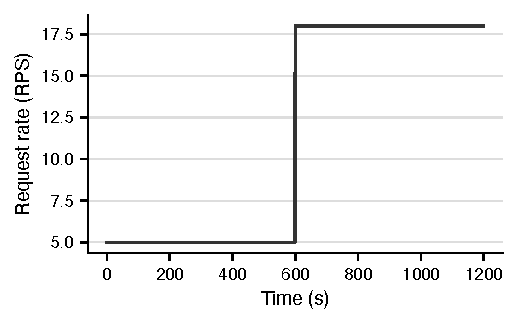
\includegraphics[width=0.32\textwidth]{../figures/workloads_eval_cpu_step.pdf}
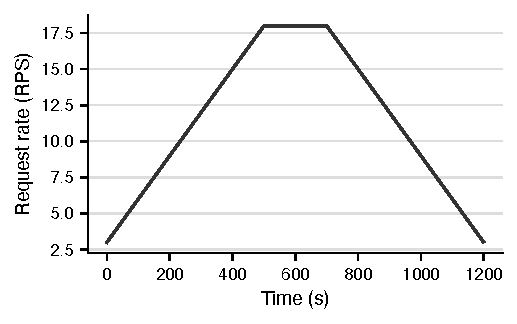
\includegraphics[width=0.32\textwidth]{../figures/workloads_eval_memory_ramp.pdf}
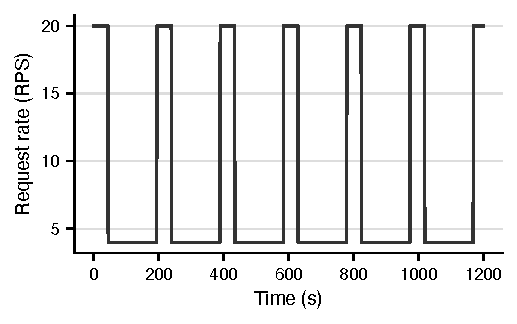
\includegraphics[width=0.32\textwidth]{../figures/workloads_eval_mixed_burst.pdf}
\caption{Request rate (RPS) versus time for the three pre-registered \texttt{eval\_\allowbreak final} profiles: \texttt{eval\_\allowbreak cpu\_\allowbreak step} (peak 18 RPS, CPU mode), \texttt{eval\_\allowbreak memory\_\allowbreak ramp} (peak 18 RPS, memory mode), \texttt{eval\_\allowbreak mixed\_\allowbreak burst} (peak 20 RPS, mixed mode).}
\label{fig:workloads}
\end{figure}

\begin{figure}[htbp]
\centering
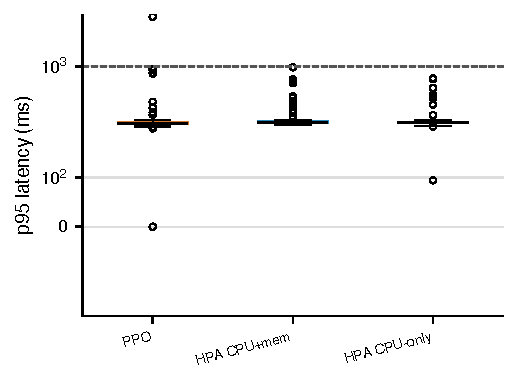
\includegraphics[width=0.42\textwidth]{../figures/evaluation_p95_boxplot_eval_cpu_step.pdf}
\caption{Box plot (symlog vertical axis, linear threshold 200\,ms) of per-decision p95 latency, pooled across 3 repeats, \texttt{eval\_\allowbreak cpu\_\allowbreak step}. Dashed line: 1000\,ms SLA target.}
\label{fig:eval-box-cpu}
\end{figure}

\begin{figure}[htbp]
\centering
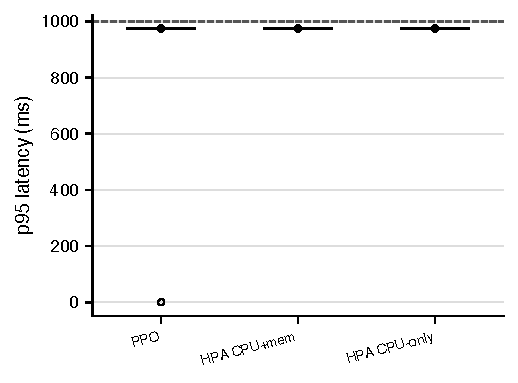
\includegraphics[width=0.42\textwidth]{../figures/evaluation_p95_boxplot_eval_memory_ramp.pdf}
\caption{Box plot (symlog vertical axis, linear threshold 200\,ms) of per-decision p95 latency, pooled across 3 repeats, \texttt{eval\_\allowbreak memory\_\allowbreak ramp}. Dashed line: 1000\,ms SLA target. The 975\,ms cluster is the histogram-bucket artefact described in the text.}
\label{fig:eval-box-memory}
\end{figure}

\begin{figure}[htbp]
\centering
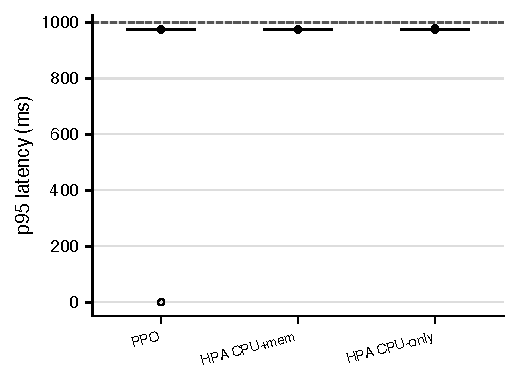
\includegraphics[width=0.42\textwidth]{../figures/evaluation_p95_boxplot_eval_mixed_burst.pdf}
\caption{Box plot (symlog vertical axis, linear threshold 200\,ms) of per-decision p95 latency, pooled across 3 repeats, \texttt{eval\_\allowbreak mixed\_\allowbreak burst}. Dashed line: 1000\,ms SLA target. The 975\,ms cluster is the histogram-bucket artefact described in the text.}
\label{fig:eval-box-mixed}
\end{figure}

Figure~\ref{fig:eval-replica-minutes} shows replica-minutes per profile
and arm with error bars (mean $\pm$ sd), and
Figures~\ref{fig:eval-replicas-cpu}-\ref{fig:eval-p95-mixed} show replica
count and p95 latency over time for the median-cost repeat of each arm on
each profile.

\begin{figure}[htbp]
\centering
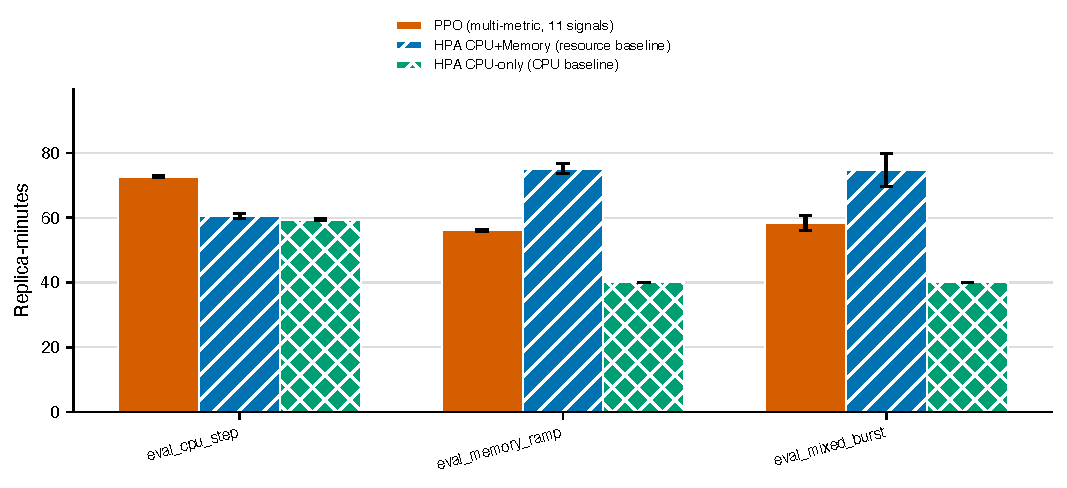
\includegraphics[width=0.42\textwidth]{../figures/evaluation_replica_minutes.pdf}
\caption{Replica-minutes (cost proxy), mean $\pm$ sd over 3 repeats, per profile and arm, \texttt{eval\_\allowbreak final}.}
\label{fig:eval-replica-minutes}
\end{figure}

\begin{figure}[htbp]
\centering
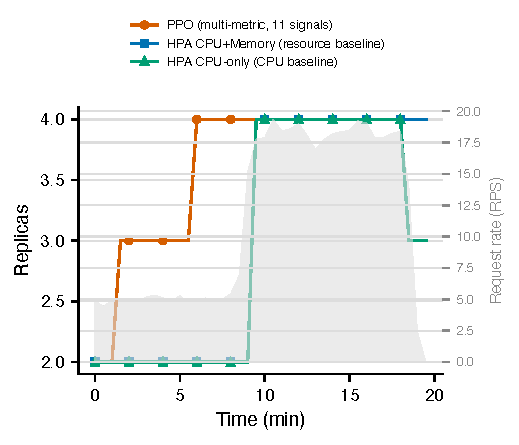
\includegraphics[width=0.42\textwidth]{../figures/evaluation_replicas_over_time_eval_cpu_step.pdf}
\caption{Replica count over time, \texttt{eval\_\allowbreak cpu\_\allowbreak step}, all 3 arms (median-cost repeat per arm), with request rate as a light background.}
\label{fig:eval-replicas-cpu}
\end{figure}

\begin{figure}[htbp]
\centering
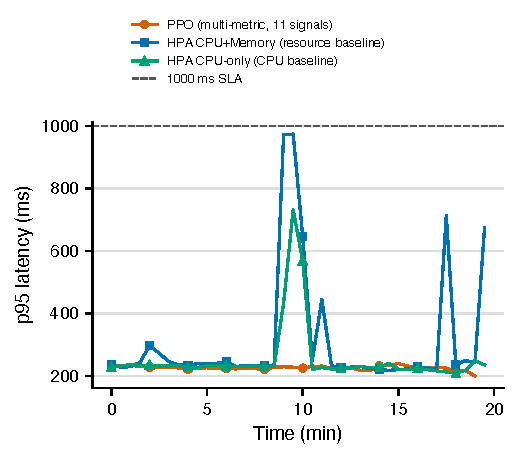
\includegraphics[width=0.42\textwidth]{../figures/evaluation_p95_over_time_eval_cpu_step.pdf}
\caption{p95 latency over time, \texttt{eval\_\allowbreak cpu\_\allowbreak step}, all 3 arms (median-cost repeat per arm), with the 1000\,ms SLA line.}
\label{fig:eval-p95-cpu}
\end{figure}

\begin{figure}[htbp]
\centering
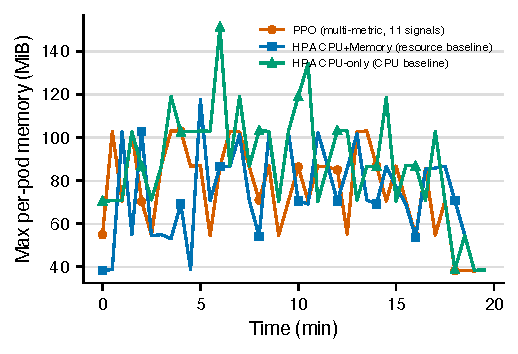
\includegraphics[width=0.42\textwidth]{../figures/evaluation_memory_over_time.pdf}
\caption{Maximum per-pod memory (MiB) over time on \texttt{eval\_\allowbreak memory\_\allowbreak ramp}, all 3 arms (median-cost repeat per arm).}
\label{fig:eval-memory-time}
\end{figure}

\begin{figure}[htbp]
\centering
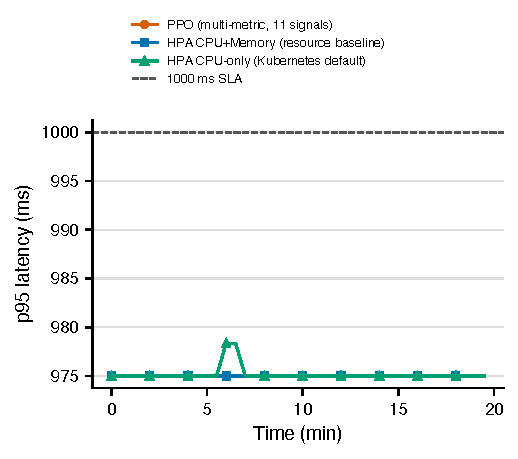
\includegraphics[width=0.42\textwidth]{../figures/evaluation_p95_over_time_eval_mixed_burst.pdf}
\caption{p95 latency over time, \texttt{eval\_\allowbreak mixed\_\allowbreak burst}, all 3 arms (median-cost repeat per arm), with the 1000\,ms SLA line.}
\label{fig:eval-p95-mixed}
\end{figure}

\subsection{PPO Policy Behaviour and Tie-Break Usage}

Across all 360 PPO decisions made during \texttt{eval\_\allowbreak final} (27 PPO
episodes $\times$ 40 decisions each, for the 9 PPO runs), HOLD was chosen
347 times, SCALE\_UP\_ONE 13 times (3.6\%), and SCALE\_DOWN\_ONE never.
Figure~\ref{fig:ppo-policy-map} shows the dominant action per
(CPU-per-replica, memory-per-replica) bin: HOLD dominates almost every
bin, and the 13 scale-up decisions are spread across a wide range of CPU
values rather than concentrated only at high CPU, suggesting the policy's
scale-up decisions are driven by more than CPU alone, consistent with its
eleven-feature, multi-signal observation space.

\begin{figure}[htbp]
\centering
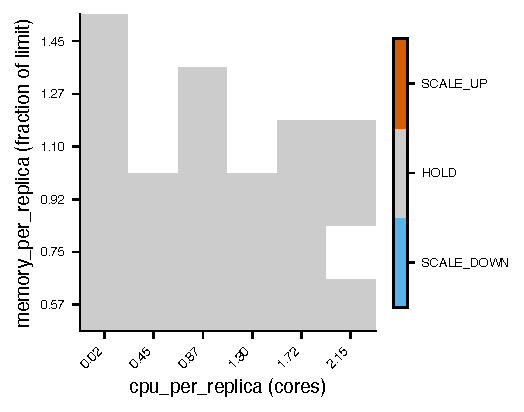
\includegraphics[width=0.42\textwidth]{../figures/discussion_ppo_policy_map.pdf}
\caption{Dominant action (SCALE\_DOWN/HOLD/SCALE\_UP) per (CPU-per-replica, memory-per-replica) bin, \texttt{eval\_\allowbreak final} PPO decisions. HOLD dominates almost every bin; only 13 of 360 decisions (3.6\%) are SCALE\_UP.}
\label{fig:ppo-policy-map}
\end{figure}

The safety-aware tie-break rule of Section~\ref{sec:tie-break} fired (that
is, an actual tie among two or more actions was detected and resolved by
rules R3-R6, not simply R1's "no tie") in exactly 4 of these 360 decisions
(1.11\%), shown in Figure~\ref{fig:tie-rule-frequency}. The rule is, by
design and in practice, a rare intervention: the overwhelming majority of
decisions have a single clear highest-probability action, and the rule
only matters at the margin.

\begin{figure}[htbp]
\centering
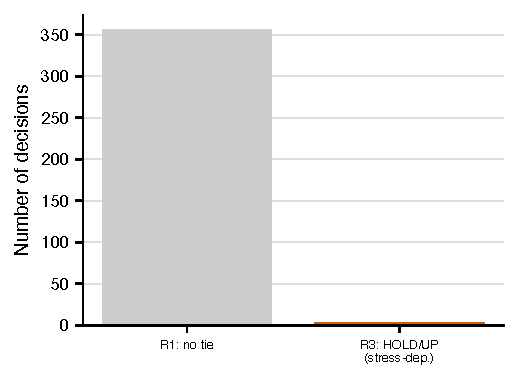
\includegraphics[width=0.42\textwidth]{../figures/discussion_tie_rule_frequency.pdf}
\caption{Frequency of each CORR-58 tie-break rule firing across \texttt{eval\_\allowbreak final} PPO decisions (R1 = no tie; R3-R6 = an actual tie resolved). An actual tie-break fired in 4 of 360 decisions (1.11\%).}
\label{fig:tie-rule-frequency}
\end{figure}

\subsection{Verdict}

Applying the pre-registered decision rule of Table~\ref{tab:decision-rule}
to the results above: the SLA-violation-rate metric produces no decidable
winner between any pair of arms on any profile, because every arm sits at
or effectively at its floor of 0.0 at this evaluation's load levels. The
replica-minutes metric does discriminate, but not in a single arm's
favour across all three profiles: the HPA CPU-only (CPU baseline) arm is
cheapest on two of three profiles and ties on the third; PPO's cost
ranking is profile-dependent, cheaper than the HPA CPU+Memory arm on two
profiles but more expensive than both HPA arms on \texttt{eval\_\allowbreak cpu\_\allowbreak step}.
No safety termination occurred in any of the 27 valid runs. Per the
pre-registration's own rule against declaring a single aggregate winner
when metrics disagree, we report this explicitly as a profile-dependent
trade-off: \textbf{no controller is declared better than the others
overall}, and the latency objective, at these evaluation-level loads,
simply does not separate the three arms.

\section{Exploratory Stress Test}

\subsection{Overview}

The exploratory \texttt{stress\_\allowbreak explore} campaign (CORR-65) was added
after \texttt{eval\_\allowbreak final}'s results already existed, specifically because
those results showed the primary SLA metric sitting at or near its floor
for every arm, unable to discriminate between controllers at
\texttt{eval\_\allowbreak final}'s light load levels. Because this addition is
explicitly outcome-aware (it was motivated by having already seen
\texttt{eval\_\allowbreak final}'s results), it is run with only one repeat per
(profile, arm) cell (9 runs total, referencing the same three profiles'
training-level-peak counterparts: \texttt{stress\_\allowbreak cpu\_\allowbreak burst},
\texttt{stress\_\allowbreak memory\_\allowbreak ramp}, \texttt{stress\_\allowbreak mixed\_\allowbreak burst}, peaking at
45-70 RPS, never beyond loads already exercised live during training) and
is reported throughout as \textbf{descriptive only}: the pre-registered
"better in all 3 repeats" decision rule cannot be and is not applied to a
single-repeat dataset, and every figure and table from this campaign is
labelled exploratory so it can never be mistaken for, or merged with, the
pre-registered \texttt{eval\_\allowbreak final} results above.

\begin{figure}[htbp]
\centering
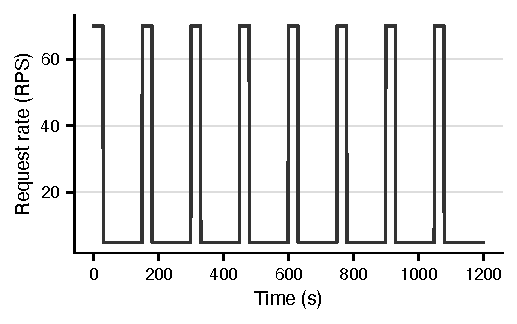
\includegraphics[width=0.32\textwidth]{../figures/workloads_stress_cpu_burst.pdf}
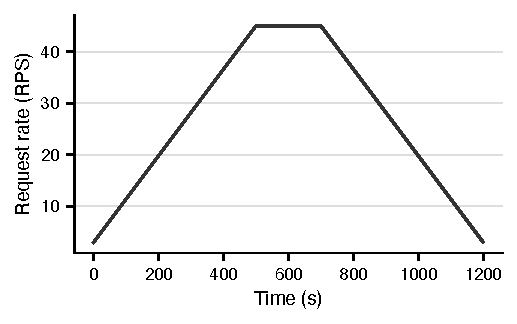
\includegraphics[width=0.32\textwidth]{../figures/workloads_stress_memory_ramp.pdf}
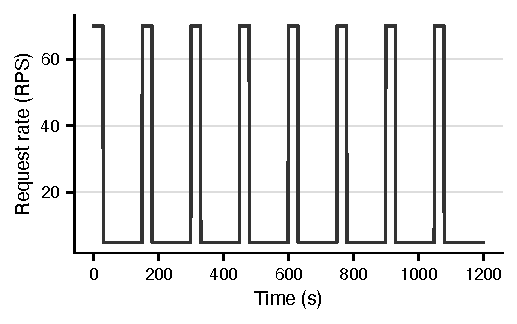
\includegraphics[width=0.32\textwidth]{../figures/workloads_stress_mixed_burst.pdf}
\caption{Request rate (RPS) versus time for the three exploratory \texttt{stress\_\allowbreak explore} profiles (CORR-65): \texttt{stress\_\allowbreak cpu\_\allowbreak burst} (peak 70 RPS), \texttt{stress\_\allowbreak memory\_\allowbreak ramp} (peak 45 RPS), \texttt{stress\_\allowbreak mixed\_\allowbreak burst} (peak 70 RPS).}
\label{fig:workloads-stress}
\end{figure}

\subsection{Descriptive Results}

Table~\ref{tab:stress-descriptive-main} reports the primary descriptive
metrics for all 9 stress runs (1 repeat each); the full table, including
secondary metrics, is given in Appendix~\ref{ch:appendix},
Table~\ref{tab:stress-descriptive-appendix}.

\begin{table}[H]
\centering
\caption{\texttt{stress\_\allowbreak explore} descriptive metrics (selected columns), 1 repeat per cell -- exploratory, CORR-65.}
\label{tab:stress-descriptive-main}
\small
\begin{tabular}{llrrr}
\toprule
Profile & Arm & SLA-viol.\ (1000\,ms) & Replica-minutes & Mean p95 (ms) \\
\midrule
stress\_cpu\_burst & HPA CPU+Memory & 0.5263 & 123.00 & 1820.3 \\
stress\_cpu\_burst & HPA CPU-only & 0.5250 & 130.00 & 1703.1 \\
stress\_cpu\_burst & PPO & 0.5000 & 84.00 & 1567.6 \\
stress\_memory\_ramp & HPA CPU+Memory & 0.0000 & 78.00 & 975.0 \\
stress\_memory\_ramp & HPA CPU-only & 0.0000 & 40.00 & 975.0 \\
stress\_memory\_ramp & PPO & 0.0000 & 56.00 & 950.6 \\
stress\_mixed\_burst & HPA CPU+Memory & 0.0000 & 76.00 & 980.3 \\
stress\_mixed\_burst & HPA CPU-only & 0.1000 & 62.50 & 1041.4 \\
stress\_mixed\_burst & PPO & 0.2000 & 66.50 & 1091.7 \\
\bottomrule
\end{tabular}
\end{table}

Under \texttt{stress\_\allowbreak cpu\_\allowbreak burst}, all three arms miss the SLA objective
roughly half the time (0.50-0.53), with PPO lowest on both cost (84.0
replica-minutes versus 123.0-130.0 for the two HPA arms) and mean p95
latency (1567.6\,ms versus 1703.1-1820.3\,ms); Figure~\ref{fig:stress-replicas-cpu}
shows why: both HPA arms repeatedly hit the 8-replica ceiling under this
profile, while PPO rises step by step to 5 replicas and holds there,
spending less on replicas while still achieving slightly lower latency.
Under \texttt{stress\_\allowbreak memory\_\allowbreak ramp}, no arm breaches the SLA at all, and
PPO's cost (56.0) sits between the HPA CPU-only arm's 40.0 and the HPA
CPU+Memory arm's 78.0. Under \texttt{stress\_\allowbreak mixed\_\allowbreak burst}, the ordering
reverses: PPO has the \emph{highest} SLA-violation rate of the three arms
(0.20, versus 0.00 for HPA CPU+Memory and 0.10 for HPA CPU-only) at a
mid-range cost (66.5) -- the opposite ordering from
\texttt{stress\_\allowbreak cpu\_\allowbreak burst}. \textbf{No single arm is uniformly better
across all three stress profiles.}

\begin{figure}[htbp]
\centering
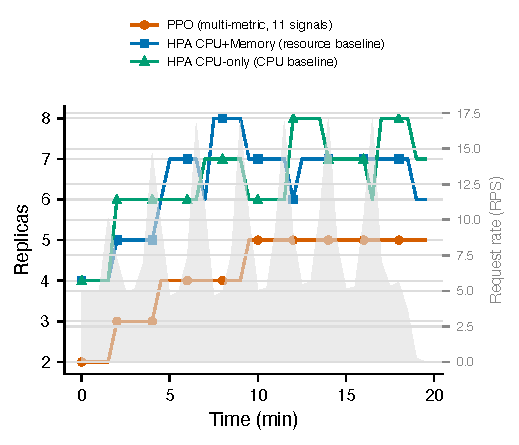
\includegraphics[width=0.42\textwidth]{../figures/stress_replicas_over_time_stress_cpu_burst.pdf}
\caption{Replica count over time, \texttt{stress\_\allowbreak cpu\_\allowbreak burst} (exploratory, CORR-65, 1 repeat per arm), with request rate as a light background. Both HPA arms repeatedly hit the 8-replica ceiling; PPO caps at 5 replicas.}
\label{fig:stress-replicas-cpu}
\end{figure}

\begin{figure}[htbp]
\centering
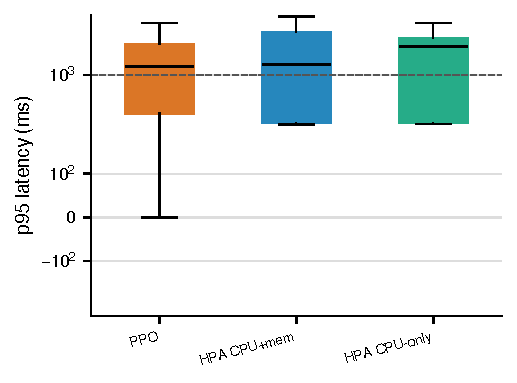
\includegraphics[width=0.42\textwidth]{../figures/stress_p95_boxplot_stress_cpu_burst.pdf}
\caption{Box plot (symlog vertical axis, linear threshold 200\,ms) of per-decision p95 latency, \texttt{stress\_\allowbreak cpu\_\allowbreak burst} (exploratory, CORR-65, 1 repeat per arm). Dashed line: 1000\,ms SLA target.}
\label{fig:stress-box-cpu}
\end{figure}

\begin{figure}[htbp]
\centering
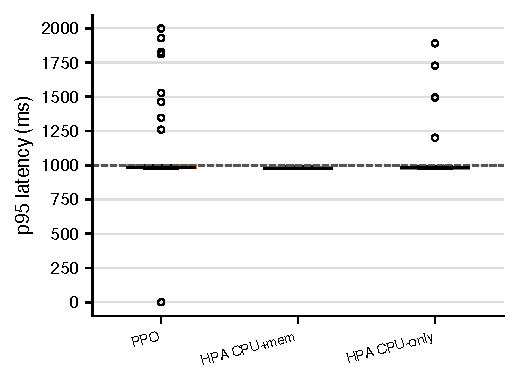
\includegraphics[width=0.42\textwidth]{../figures/stress_p95_boxplot_stress_mixed_burst.pdf}
\caption{Box plot (symlog vertical axis, linear threshold 200\,ms) of per-decision p95 latency, \texttt{stress\_\allowbreak mixed\_\allowbreak burst} (exploratory, CORR-65, 1 repeat per arm). Dashed line: 1000\,ms SLA target. PPO shows a wider spread above the SLA line than either HPA arm here, consistent with its higher SLA-violation rate on this profile.}
\label{fig:stress-box-mixed}
\end{figure}

\begin{figure}[htbp]
\centering
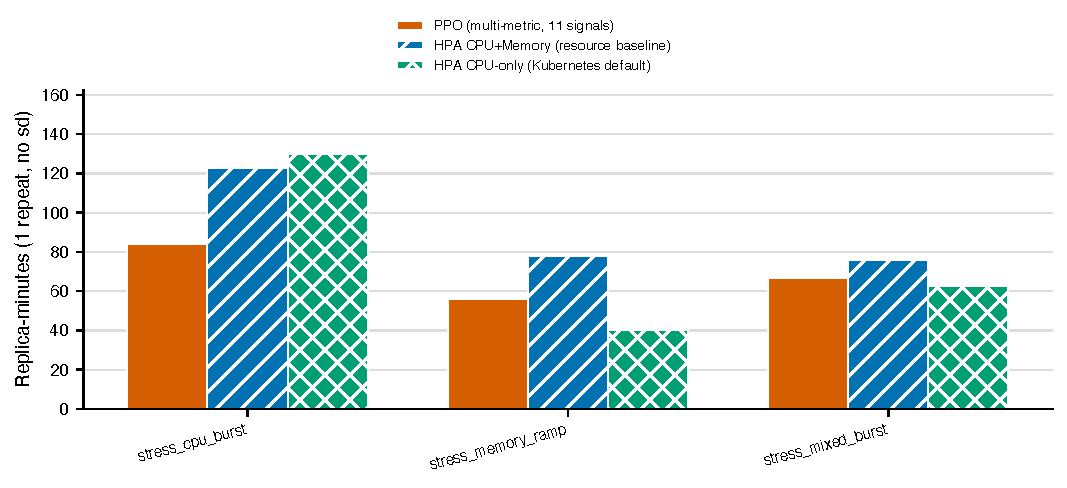
\includegraphics[width=0.42\textwidth]{../figures/stress_replica_minutes.pdf}
\caption{Replica-minutes (cost proxy), 1 repeat per cell (no error bars), per profile and arm, \texttt{stress\_\allowbreak explore} (exploratory, CORR-65).}
\label{fig:stress-replica-minutes}
\end{figure}

Figure~\ref{fig:cost-vs-latency} places every run from both campaigns on a
single cost-versus-latency plot: the exploratory stress-test points sit
well above and to the right of the \texttt{eval\_\allowbreak final} cluster, showing
that both cost and latency rise together once load moves from
\texttt{eval\_\allowbreak final}'s light levels to training-level peaks.

\begin{figure}[htbp]
\centering
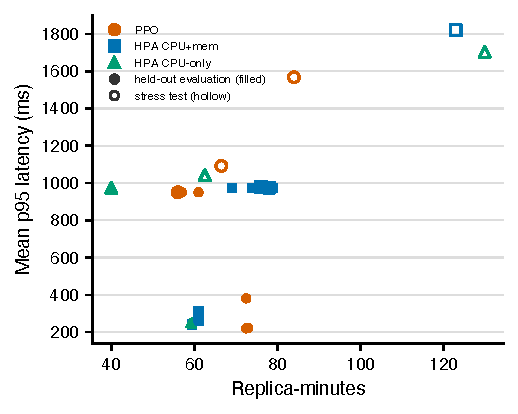
\includegraphics[width=0.42\textwidth]{../figures/discussion_cost_vs_latency.pdf}
\caption{Replica-minutes (x-axis) versus mean p95 latency (y-axis), one point per run; \texttt{eval\_\allowbreak final} points filled, \texttt{stress\_\allowbreak explore} points hollow.}
\label{fig:cost-vs-latency}
\end{figure}

\section{Comparative Analysis Against Related Work}
\label{sec:comparative-analysis}

Returning to Table~\ref{tab:related-work-summary} in
Chapter~\ref{ch:introduction}: the studies we surveyed that report
favourable RL-versus-baseline comparisons (Mao et al.\
\cite{mao2016resource}, Rossi et al.\ \cite{rossi2019horizontal}, Imdoukh
et al.\ \cite{imdoukh2020lstm}, Qiu et al.\ \cite{qiu2020firm}) train
and/or evaluate primarily in a simulator or against a recorded trace, and,
as far as we could establish from their published descriptions, do not
report a baseline comparison whose protocol and decision rule were fixed
in writing before any evaluation result existed. Our project differs on
both counts: every decision step, in both V1 and V2, training and
evaluation, was executed against a real Minikube cluster, and our V2
evaluation protocol, metrics, and decision rule were pre-registered
(CORR-60) before the final training checkpoint existed. This difference
has a direct, visible cost: our sample sizes (three repeats per
pre-registered cell, one per exploratory cell) are far smaller than a
simulator-based study could collect in the same wall-clock time, and our
results are correspondingly more cautious -- we report a profile-dependent
trade-off rather than a clean win, where some of the surveyed simulator-
or trace-based work reports a clear improvement over its baseline. We
think this trade-off, smaller but harder-won samples against a real
system versus larger but simulated samples, is a genuine trade-off rather
than a flaw unique to our approach, and it is consistent with the point
Henderson et al.\ \cite{henderson2018matters} and Dulac-Arnold et al.\
\cite{dulacarnold2019challenges} make about how much harder reliable RL
evaluation becomes once a real system, rather than a simulator, is in the
loop.

\section{Discussion}
\label{sec:discussion}

Three threads tie the V1 and V2 results together. First, V1's failure and
V2's redesign are a single, connected story, not two separate projects:
every major V2 design change in Table~\ref{tab:v1-v2-comparison} traces
directly to a specific, nameable problem observed in V1's evaluation or
training, and the honesty of reporting V1's failure in full
(Section~\ref{sec:v1-failure}) is what makes the V2 redesign's rationale
legible rather than asserted. Second, V2's training curves
(Section~\ref{sec:zero-ready-stops} and Figures~\ref{fig:training-reward}-\ref{fig:training-action-mix})
show a policy that was still improving, not one that had clearly
plateaued, by session 47: entropy loss and explained variance both
continue to move in the expected direction through the last few sessions
rather than flattening out well before the campaign's end, which is part
of why we list a longer training budget as future work
(Section~\ref{ch:conclusion}) rather than treating 12,288 timesteps as
necessarily sufficient. Third, and most directly tied to our stated
problem statement, the pre-registered evaluation's "ceiling effect" -- the
primary SLA metric sitting at or near zero for every arm at
\texttt{eval\_\allowbreak final}'s load levels -- is not a flaw we discovered after
the fact and tried to explain away; it is the direct, literal reason the
exploratory stress test exists at all, and the stress test's own finding
(no single arm uniformly better across stress profiles either) means that
moving to a harder evaluation load did not resolve the ambiguity in PPO's
favour, or in either HPA arm's favour -- it only showed that each
controller's relative strength depends on which resource dimension is
under pressure.

\section{Limitations}
\label{sec:limitations}

We list our limitations plainly rather than treating them as minor
caveats.

\begin{itemize}[nosep]
  \item \textbf{Light evaluation loads / ceiling effect.} The three
    pre-registered \texttt{eval\_\allowbreak final} profiles peak at 18-20 RPS, well
    below the 45-70 RPS peaks exercised live during training. At this
    light load, the primary SLA metric sits at or near its floor (about
    0) for every arm, so it cannot discriminate between controllers under
    \texttt{eval\_\allowbreak final} specifically; the exploratory stress test was
    added, after the fact, to probe heavier loads, but remains a
    descriptive, one-repeat addition and does not substitute for a
    pre-registered, three-repeat evaluation at higher load.
  \item \textbf{Single-repeat stress test.} Every \texttt{stress\_\allowbreak explore}
    number is a single observation, not a mean over repeats, and cannot
    support the pre-registered better-in-all-three-repeats decision rule;
    we report it descriptively for exactly this reason.
  \item \textbf{Histogram-bucket artefact.} A recurring p95 latency value
    of exactly 975\,ms, seen across several \texttt{eval\_\allowbreak memory\_\allowbreak ramp}/
    \texttt{eval\_\allowbreak mixed\_\allowbreak burst}/stress cells for every arm, is a
    Prometheus histogram-bucket interpolation artefact, not a precisely
    measured value -- the true p95 lies somewhere in the 500-1000\,ms
    bucket range, and we do not report it as more precise than that.
  \item \textbf{Single-node local cluster.} All training, evaluation, and
    stress-test runs executed on a single-node Minikube cluster (Docker
    driver) on one laptop, not a multi-node, production-scale cluster;
    absolute resource headroom, scheduling behaviour, and node-level
    contention may differ on a larger cluster.
  \item \textbf{Two failed-and-retried training sessions.} Sessions 4 and
    38 of the 48-session V2 training campaign failed on
    \texttt{zero\_\allowbreak ready\_\allowbreak replicas} and were retried under this project's
    resume discipline (Section~\ref{sec:zero-ready-stops}); the 48
    analyzed sessions are the successful retries, not a silently dropped
    or averaged-over failure, and both are marked explicitly in every
    training-curve figure.
  \item \textbf{Grafana disabled during V2 evaluation.} Grafana was scaled
    to zero replicas for the entire V2 evaluation campaign
    (Section~\ref{sec:eval-protocol}) so that it could not compete with
    the benchmark application for the Minikube node's limited CPU and
    memory, or add confounding load during a measured run. This means no
    live Grafana dashboard was available to monitor runs visually during
    evaluation; all telemetry used for analysis came directly from
    Prometheus, not from Grafana.
  \item \textbf{Small sample sizes.} Three repeats per pre-registered cell
    and one repeat per exploratory cell are both small by the standards
    Agarwal et al.\ \cite{agarwal2021precipice} argue for in RL evaluation
    generally; we report means and standard deviations rather than single
    point estimates wherever more than one repeat exists, but we do not
    claim statistical power beyond what three (or one) repeats can
    support.
  \item \textbf{Operational incidents during V2.} Two training sessions
    failed and were retried (above); four \texttt{eval\_\allowbreak final} attempts
    failed closed on a leftover HPA object and were retried once each
    (CORR-63, CORR-64) with no effect on the measured result. A host
    restart occurring specifically during the V2 evaluation campaign, and
    a training re-run ended by an external kill signal rather than by the
    \texttt{zero\_\allowbreak ready\_\allowbreak replicas} condition, are two events we were asked
    to disclose; our own search of the project's documentation located a
    closely related event (the training process at session 4 being found
    unexpectedly absent, Section~\ref{sec:zero-ready-stops}, attributable
    to the recorded \texttt{zero\_\allowbreak ready\_\allowbreak replicas} stop rather than
    confirmed as an external kill) and a host restart documented during an
    earlier, unrelated pre-training diagnostic phase, not during the
    final evaluation campaign itself. We were not able to independently
    verify an externally-killed training re-run or an evaluation-time host
    restart as separate, confirmed incidents in the materials available to
    us, and we flag this explicitly as \textbf{[CHECK]} rather than assert
    either occurred without a located record.
  \item \textbf{\texttt{reaction\_\allowbreak time\_\allowbreak s} unavailable.} This secondary
    metric is reported as \texttt{n/\allowbreak \allowbreak a} throughout our evaluation tables;
    our analysis script found no usable signal for it in the normalized
    series schema used for \texttt{eval\_\allowbreak final} and
    \texttt{stress\_\allowbreak explore}, and we report it as missing rather than
    fabricating or imputing a value.
\end{itemize}
